\documentclass[12pt, a4paper]{article}
\usepackage{times}
\usepackage{lipsum}
\usepackage[margin=1in]{geometry}
\usepackage{fancyhdr}
\usepackage{multicol}
\usepackage{graphicx}
\usepackage[font=small,labelfont=bf]{caption}
\usepackage{hyperref}
\pagestyle{fancy}
\pdfinfo{/Title Observations of the Cygnus Loop’s Supernova Remnants /Author Rei Johnson /Keywords Observation, Cygnus, Veil,
Nebula }
\setcounter{secnumdepth}{1}
\title{Observations of the Cygnus Loop’s Supernova Remnants}
\author{Rei Johnson$^{1, 2}$ \and Collaborator$^{x,x}$}
\date{%
	$^1$Department of Mathematics, Montgomery College\\%
	$^2$Department of Engineering, Physical, and Computer Sciences, Montgomery College\\[2ex]%
	\today
}
\rhead{Johnson et al.}
\lhead{Submeter Cyg. Loop Observations}

\begin{document}
% TITLE PAGE
\maketitle
\newpage

\centering
\section[bold]{Abstract}

\raggedright

\lipsum[1]

\centering
\section[bold]{Methods}

\begin{multicols*}{2}
\input
\raggedright

\subsection[bold]{2.1 Alnitak Observatory 0.43m Images}
Preliminary observations were made with the 0.43m 'A1' telescope at Alnitak Observatory (MPC I79). The A1 optical tube is a 0.43m CDK17 Correct Dall-Kirkham designed by PlaneWave Instruments (Alnitak). The telescope is equipped with a Moravian Instruments C3-61000 Pro CCD imager (Alnitak). Images taken through the A1 telescope were imaged using LRGB and OIII, H-Alpha and SII filters. The initial LRGB exposures totaled 1200 seconds of CCD exposure (4x300s) and the H-Alpha, OIII, and SII filter exposures totaled 900 seconds (3x300s).\footnote{H-Alpha, OIII, and SII filters operate on 5nm Narrowband} Primary exposures (LRGB) resulted in star-dense images, with gas-containing images being nearly exclusive to Red filter and Luminance filter images. \ref{fig1}, \ref{fig2}

\subsection[bold]{2.2 Hubble Images}
\end{multicols*}

\bibliography{Bibliography-File}
\bibliographystyle{flairs}

\begin{center}
\begin{minipage}{0.48\linewidth}
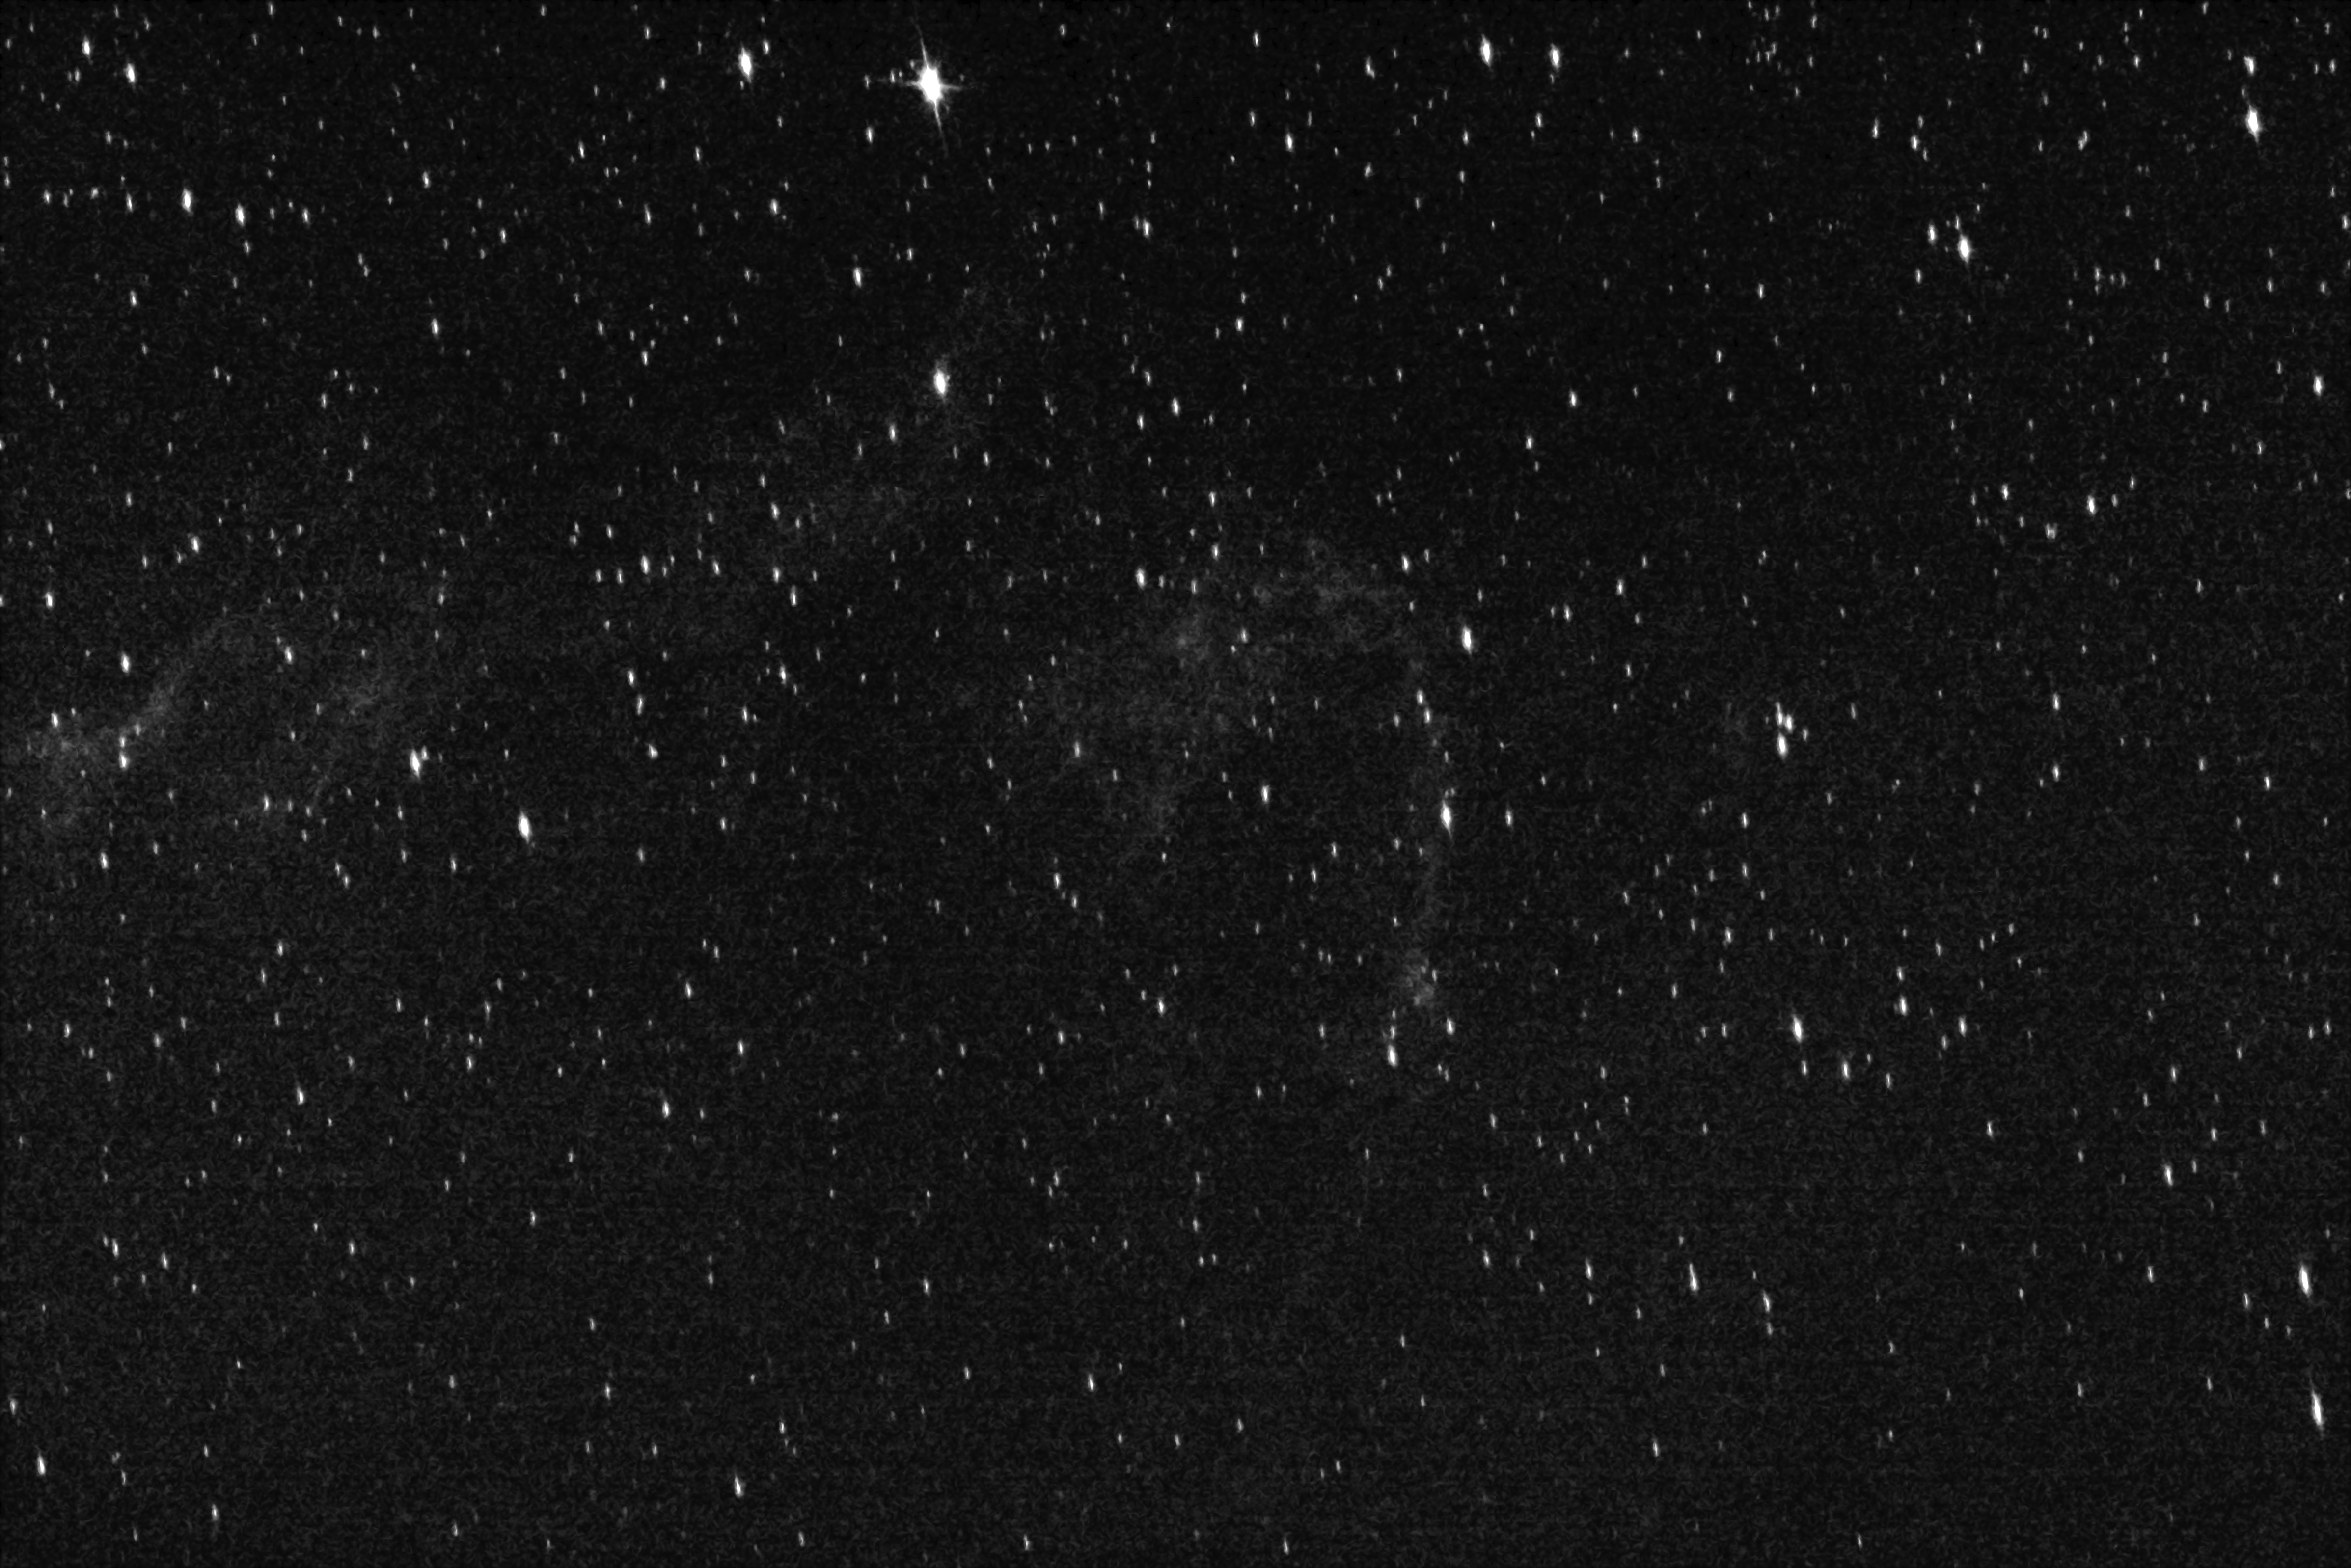
\includegraphics[width=\linewidth]{fig/red300s.jpg}
\captionof{figure}{300 second Red-filter exposure of NGC 6995}
\label{fig1}
\end{minipage}
\hfill
\begin{minipage}{0.49\linewidth}
\includegraphics[width=\linewidth]{fig/lum300s.jpg}
\captionof{figure}{300 second Luminance-filter exposure of NGC 6995}
\label{fig2}
\end{minipage}
\end{center}
\end{document}